\chapter{Final Evaluation}
\label{chap:technical-evaluation}
\vspace{-0.75cm}
\centerline{\rule{149mm}{.02in}}
\vspace{0.75cm}

Chapter \ref{chap:performance-evaluation} showed that the point $kd$-tree greatly outperforms the Pyramid Tree and Pseudo-Pyramid Tree with the two scientific datasets.
The Pseudo-Pyramid Tree has not been explored in the literature, so there were no expectations of its performance. However, it was hypothesised that the Pyramid Tree would perform better than the point $kd$-tree, which is not the case.

This chapter explores the reasons for this, determining which properties in the astrophysics dataset cause the performance of the Pyramid Tree to degenerate. The chapter concludes by discussing the suitability of the Pyramid Tree, $kd$-tree and different classes of index structures for high-dimensional scientific datasets.

\section{Characteristics of Astrophysics Dataset}
\label{sec:data-characteristics}

A dataset can be considered \textit{skewed} if there are more points in some regions of the data space than others. In other words, the underlying frequency or probability distribution of point locations is non-uniform. Intuitively, the skewness of a dataset increases as the \textit{difference} between the frequency, or probability, of points in different spatial regions increases.

Histograms are used to visualise the frequency distributions of one-dimensional data. Since this project deals with multi-dimensional data, multiple histograms, one for each dimension, can be produced to gain insight into point distribution. The astrophysics dataset was computed using a 3D sampling lattice, computing ten fields at each point. The original simulation uses interpolation to compute the ten fields at each point on the lattice \cite{astrophysics-dataset}. Carr et al. discusses how this interpolation ``implicitly applies the spatial relation between sample points" and shows that histograms are equivalent to nearest-neighbour interpolation \cite{histograms-and-isosurfaces}. This means histograms poorly represent datasets that use higher-order interpolants (like the astrophysics dataset) because the technique ``over-emphasizes densely-sampled regions and under-emphasizes sparsely-sampled regions" \cite{histograms-and-isosurfaces}. 

Isosurface statistics have been proposed as a superior representation of such datasets \cite{histograms-and-isosurfaces}. However, they are conceptually and computationally more complex to compute. Due to the project's time constraints, isosurface statistics will not be used. While histograms are a poorer representation of the data, the aim of this evaluation is to determine how skewed the data space is. Histograms still allow for this even if they are not as accurate at representing the data as other techniques. For these reasons, histograms are used to visualise the distribution of the astrophysics dataset.

\begin{figure}
	\begin{center}
		\begin{subfloat}[Dimension 1 (total particle density)]{%
			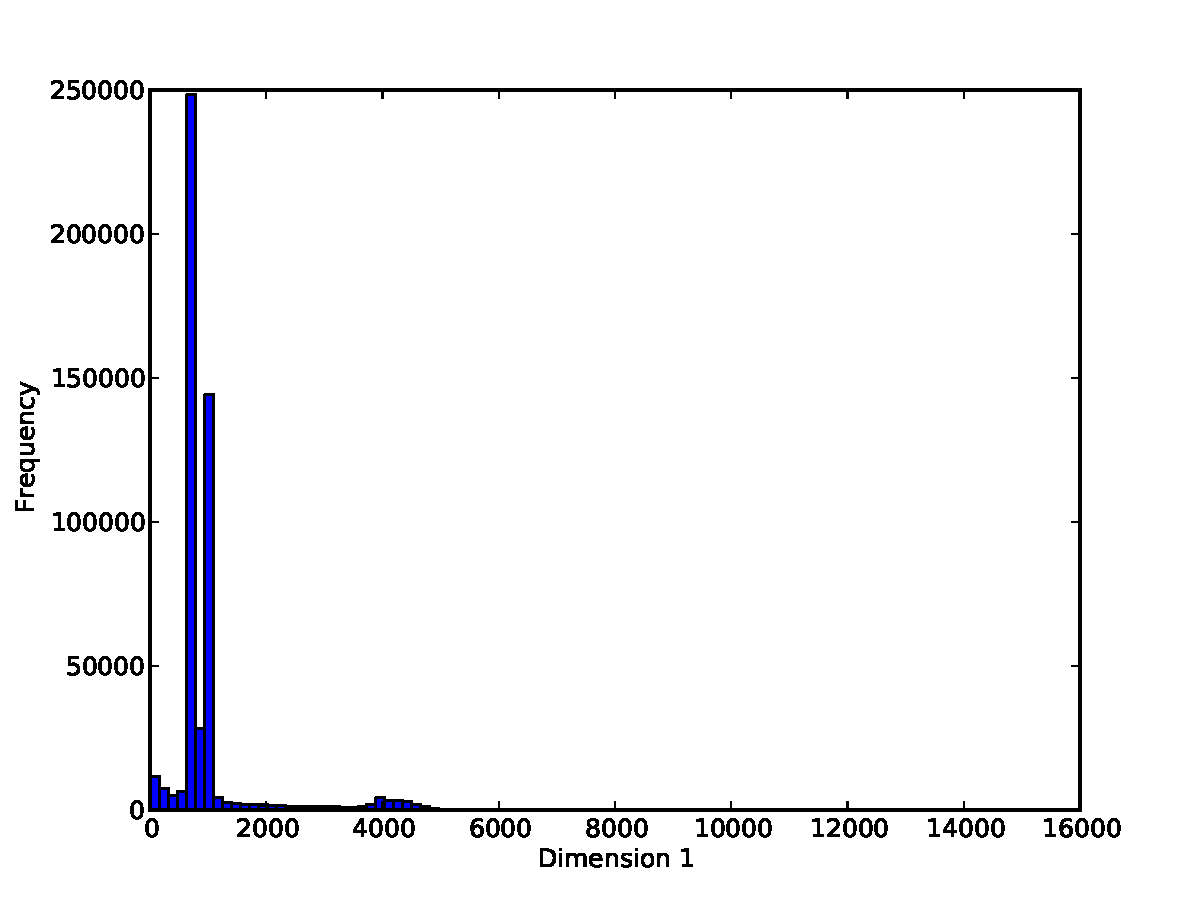
\includegraphics[scale=0.36]{figures/histograms/astrophysics_500000_0.pdf}
		}
		\end{subfloat}~
		\begin{subfloat}[Dimension 2 (gas temperature)]{%
			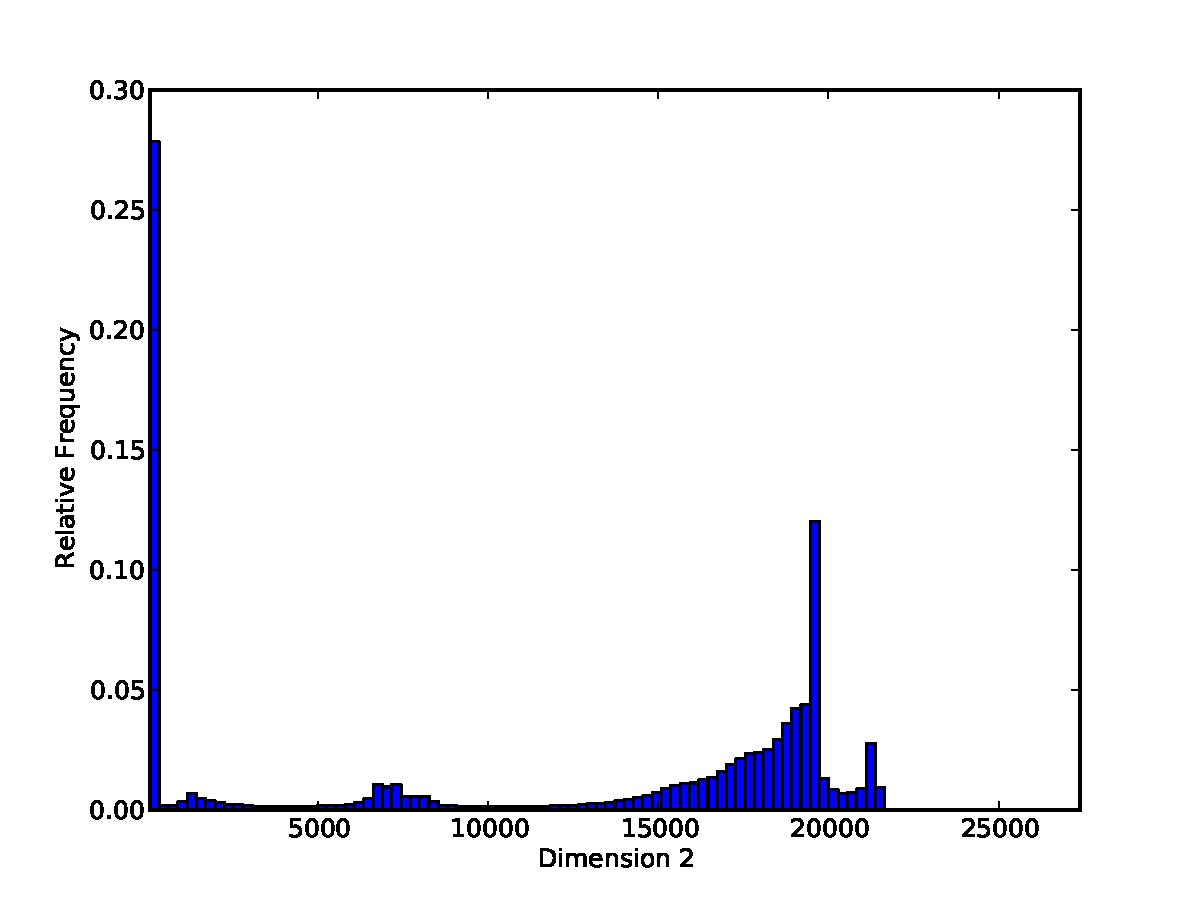
\includegraphics[scale=0.36]{figures/histograms/astrophysics_500000_1.pdf}
		}
		\end{subfloat}
	\end{center}

	\caption{Frequency Distributions of Dimensions 1 and 2 of Astrophysics Dataset}
	\label{fig:astrophysics-histograms1}
\end{figure}

\begin{figure}
	\begin{center}
		\begin{subfloat}[Dimension 3 (H mass abundance)]{%
			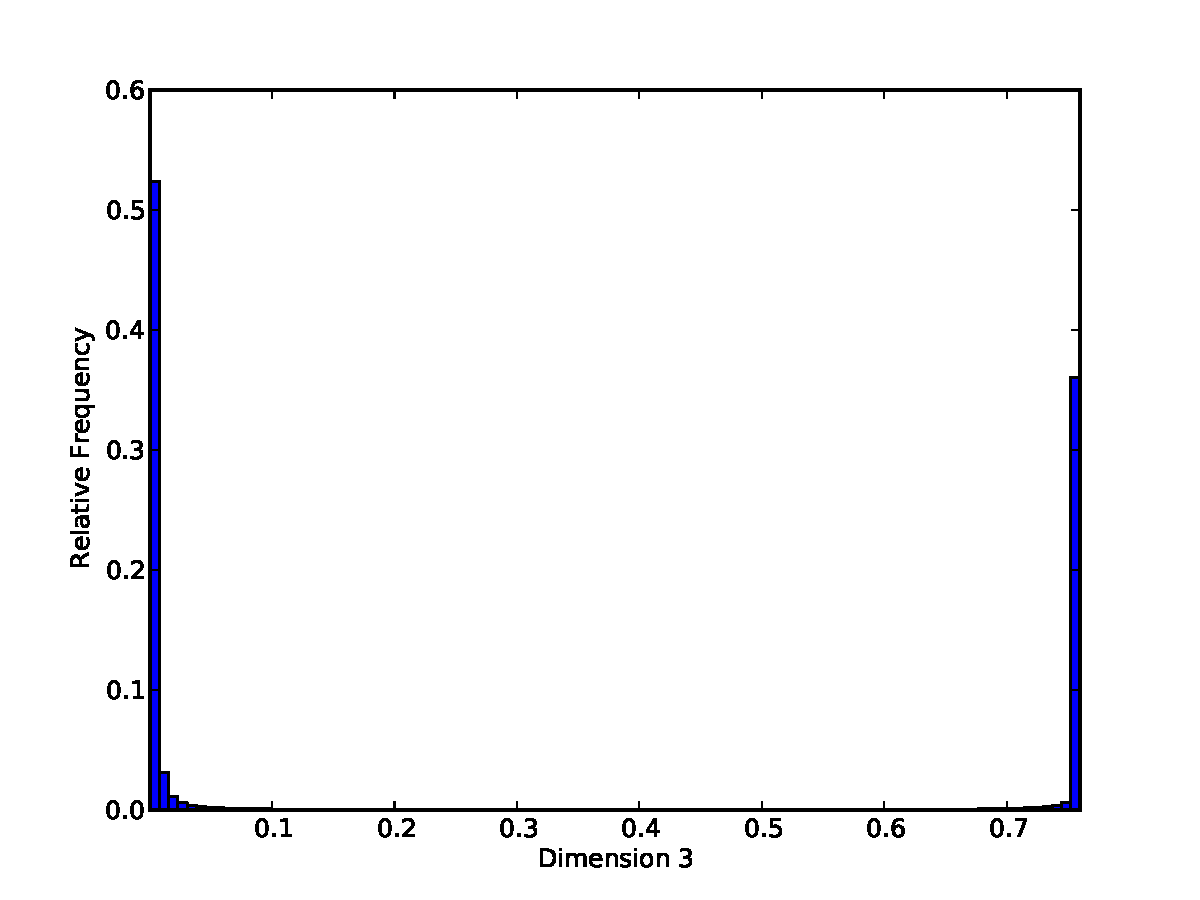
\includegraphics[scale=0.36]{figures/histograms/astrophysics_500000_2.pdf}
		}
		\end{subfloat}~
		\begin{subfloat}[Dimension 7 (He${}^{++}$ mass abundance)]{%
			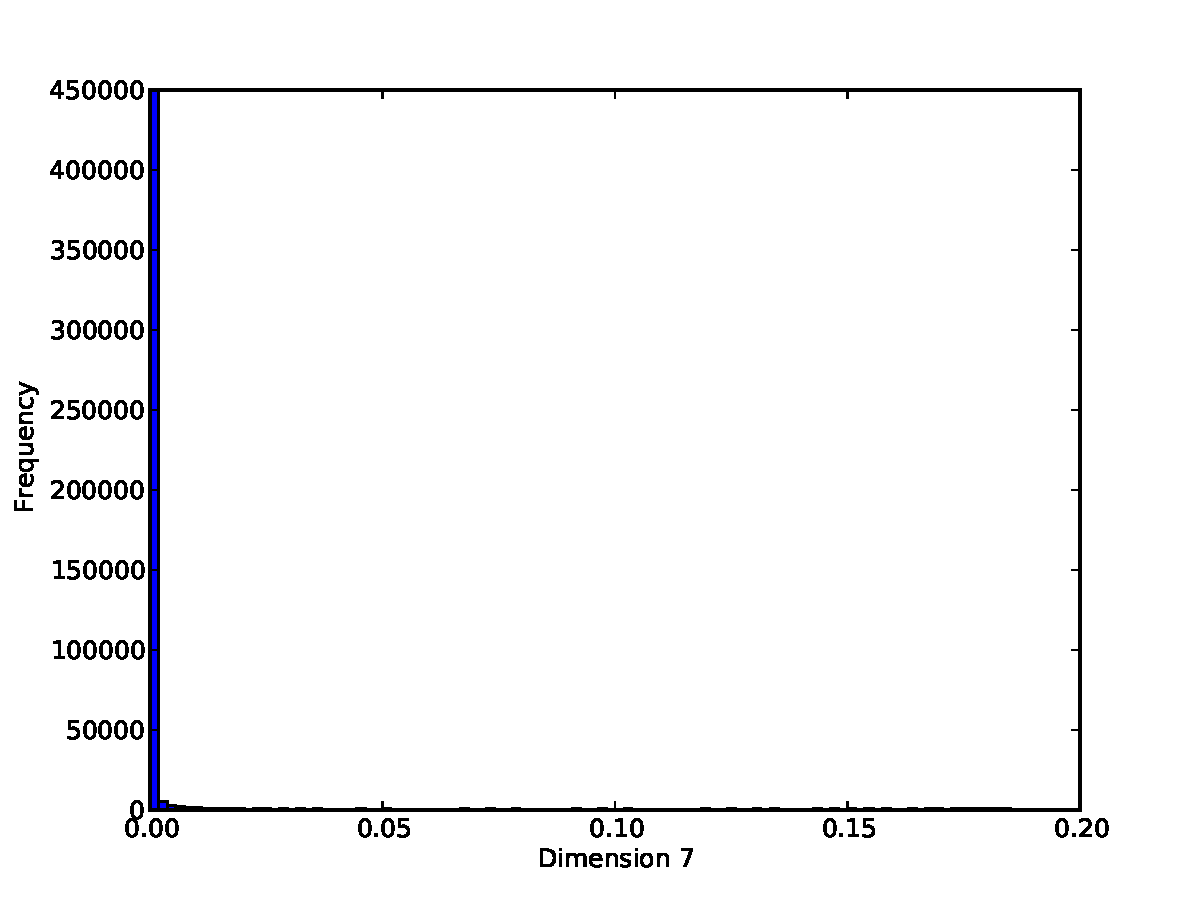
\includegraphics[scale=0.36]{figures/histograms/astrophysics_500000_6.pdf}
		}
		\end{subfloat}
	\end{center}

	\caption{Frequency Distributions of Dimensions 3 and 7 of Astrophysics Dataset}
	\label{fig:astrophysics-histograms2}
\end{figure}

Using the same sampled astrophysics dataset used for performance analysis in Chapter \ref{chap:performance-evaluation}, a histogram has been generated for each of the ten dimensions. Figures \ref{fig:astrophysics-histograms1} and \ref{fig:astrophysics-histograms2} show histograms of dimensions 1, 2, 3 and 7, where bin height represents the \textit{relative} frequency of values inside the bin. The remaining dimensions have distributions similar to the dimensions shown here, so they add little value to the discussion. They can be found in Appendix \ref{sec:app-histograms} for completeness. Using these histograms, the following observations can be made:
\begin{enumerate}
	\item the first two dimensions, total particle density and gas temperature, appear to have the greatest variance, although there are still large peaks
	\item most points are clustered at the lower or upper boundaries of dimensions 3, 4, 5 and 6. The respective histograms have massive peaks at either end of the distribution
	\item most points are clustered at the lower boundary of dimensions 7, 8, 9 and 10
\end{enumerate}
Therefore, the astrophysics dataset is highly skewed because most points are clustered at the boundaries of a dimension, and the data space is \textit{sparse} because the majority of it has little to no points.

\section{Effects of Data Distribution}

We now explore the effects of the astrophysics dataset's distribution on the Pyramid Tree and $kd$-Tree.

\subsection{Pyramid Tree}

Recall that the Pyramid Tree maps a point $v$ to a scalar value, called the point's pyramid value. Points with the same pyramid value are stored in the same bucket. Table \ref{tab:final-bucket-size} shows bucket size statistics and how long it takes to query all the points for the sampled astrophysics dataset with different subsets of dimensions. When the dimensions with the least skew (dimensions 1 and 2) are used, average bucket size decreases substantially. Dimensions 3 and 7 have large clusters of points at the boundaries, so they cause the average bucket size to increase.

The histograms from Section \ref{sec:data-characteristics} illustrate how most points lie on, or close to, the boundaries of the dataset. This is a significant problem for the Pyramid Tree because it always chooses the dimension whose distance from the centre point of the space is the highest. If a large number of points are on a dimensional boundary, then its likely the same dimension will be chosen. Each point will the same coordinate value for the chosen dimension because they are on the same boundary, meaning will have the same pyramid value and will be mapped to the same bucket.

\begin{table}
	\centering
	\makebox[\textwidth][c]{%
		\begin{tabular}{|l|l|l|l|l|}
			\hline
			& & \multicolumn{3}{c|}{\textbf{Bucket Statistics}} \\
			\hline
			\textbf{Dimensions} & \textbf{Time to Query (sec)} & \textbf{Average} & \textbf{Max} & \textbf{\#Buckets} \\
			\hline
			All & 60.0216 & 3586.57 & 235260 & 120 \\
			1 and 2 & 0.0713558 & 6.52433 & 102 & 25232 \\
			3 and 7 & 8.30587 & 89.2853 & 141235 & 3056 \\
			\hline
			No Boundary Coordinates & 27.6034 & 25.3722 & 45031 & 16963 \\
			\hline
		\end{tabular}
	}%
	\caption{Pyramid Tree Bucket Size Statistics with Different Dimensions of Astrophysics Dataset}
	\label{tab:final-bucket-size}
\end{table}

Histograms are equivalent to nearest-neighbour interpolation, so they do not show if points inside the bins at the boundary of the histograms are actually boundary values or just \textit{close} to the boundary.

To determine if clusters of points at boundaries is truly the main cause of large buckets, a heuristic called \textbf{No Boundary Coordinates} was developed. Let $v$ be a point and $min_i$ and $max_i$ be the minimum and maximum boundary values for dimension $i \in \lbrace 0, 1, ..., d - 1 \rbrace$. Let $j$ be the dimension $v$ is furthest away from the centre point with. If $v_j = min_j$ or $v_j = max_j$, then a new dimension $k$ is chosen, such that $v_k$ is the \textit{second} furthest coordinate from the centre point. If $v_k$ is at the boundary, then the \textit{third} furthest coordinate is chosen. This process is repeated until a coordinate which is not on a boundary is found. If all coordinates are on a boundary, then the first dimension is chosen.

Table \ref{tab:final-bucket-size} shows how this simple heuristic decreases average bucket size. However, it is still significantly slower than the $kd$-tree, so boundary points are not the only problem with the dataset. Note that creating heuristics like this requires pre-existing knowledge of the point distribution, which may not be available, especially when the data is dynamic (i.e. all the points are not known in advance).

\subsection{$kd$-Tree}

Table \ref{tab:final-balance-factor} shows point $kd$-tree query time, balance factor and maximum path length of the tree with different dimensions of the astrophysics dataset. It can be observed that the point $kd$-tree, like the Pyramid Tree, performs worse because of the skew present in the astrophysics dataset. Using dimensions 1 and 2 gives a lower balance factor than the more skewed dimensions 3 and 7.

The performance difference between each dimension subset is much smaller than the Pyramid Tree, again showing that the point $kd$-tree is more resilient to skew than the Pyramid Tree.

\begin{table}
	\centering
	\makebox[\textwidth][c]{%
		\begin{tabular}{|l|l|l|l|l|}
			\hline
			\textbf{Dimensions} & \textbf{Time to Query (sec)}  & \textbf{Balance Factor} & \textbf{Max Path Length}  \\
			\hline
			All & 0.639265 & 32.405 & 120 \\
			1 and 2 & 0.18445 & 26.5923 & 73 \\
			3 and 7 & 0.257211 & 28.6481 & 69 \\
			\hline
		\end{tabular}
	}%
	\caption{Point $kd$-tree Statistics with Different Dimensions of Astrophysics Dataset}
	\label{tab:final-balance-factor}
\end{table}

\section{Conjecture on Scientific Datasets}

While an analysis of the hurricane Isabel dataset is not in this report, generating histograms of each dimension reveals distributions similar to the astrophysics dataset. Some dimensions have smoother distributions, whereas others contain large clusters of points at the boundaries. This raises an important question: do datasets resulting from scientific simulations generally have these properties, or are these properties just specific to these datasets? If the former is true, more general hypotheses can be made regarding which index structures are suitable for scientific computation and visualisation.

Exploring the properties of scientific multi-dimensional datasets is a project in itself, so an in-depth analysis of such properties is not performed. Instead, a conjecture regarding point distributions of scientific datasets will be given. The reasoning behind this conjecture will then be discussed.

\paragraph{\textbf{CONJECTURE:}} Highly clustered and sparse data spaces is a property held by the majority of scientific datasets computed using sampled lattices.
\paragraph{}

Scientific datasets are often computed using $m$-dimensional sampling lattices, where each point on the lattice represents a point in physical space. The astrophysics dataset was computed in this way. \cite{astrophysics-dataset}. $m$ is usually 2 or 3, because \textit{physical} phenomena is typically being simulated. $d$ continuous fields are measured at each point, which are typically physical properties such as temperature, wind velocity, chemical masses and so on. Interpolation is applied to model the \textit{spatial} relationships between the sampling points in physical space.

It is common for $d$ to be larger than $m$, like the astrophysics and hurricane Isabel datasets. These physical simulations can be described as a mapping $\mathbb{R}^m \rightarrow \mathbb{R}^d$, where $d > m$. As $d$ increases, the data space's volume increases exponentially, resulting in greater sparsity (as discussed in Section \ref{sec:curse-of-dimensionality}).

Data sparsity becomes an even greater issue when mapping continuous domains to higher dimensional space because the resulting $d$-dimensional dataset becomes a sampled $m$-manifold in $d$-dimensional space. Figure \ref{fig:manifolds} illustrates examples of manifolds for $\mathbb{R}^1 \rightarrow \mathbb{R}^2$ and $\mathbb{R}^2 \rightarrow \mathbb{R}^3$. Notice how the majority of the data spaces are empty in both examples. Only thin strips of the data spaces are filled by the lower-dimensional manifolds. The astrophysics dataset was the result of a $\mathbb{R}^3 \rightarrow \mathbb{R}^{10}$ simulation, so a 3 dimensional manifold is embedded in 10 dimensional space. The resultant 10D space is highly sparse, which would explain why there are huge clusters in the astrophysics dataset.

\begin{figure}
	\begin{center}
		\begin{subfloat}[$\mathbb{R}^1 \rightarrow \mathbb{R}^2$]{%
			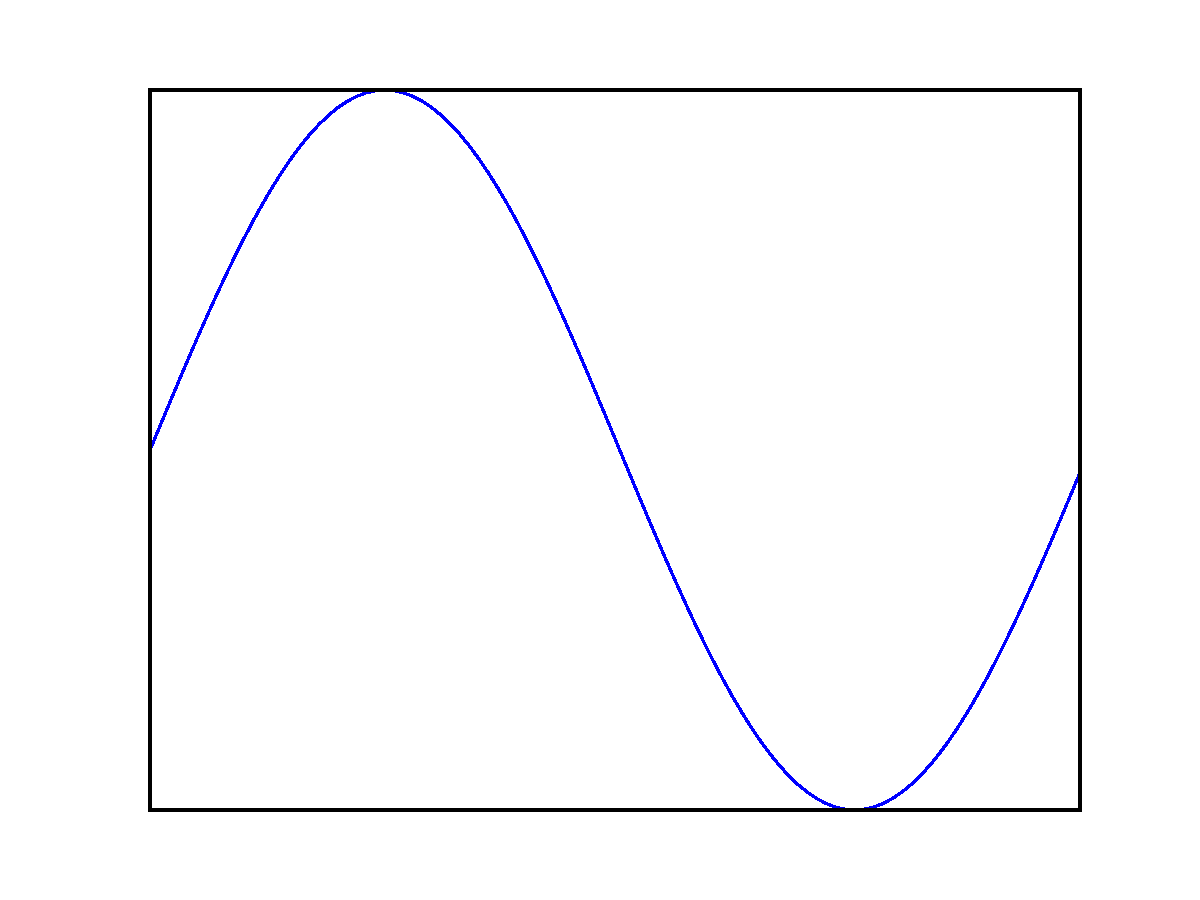
\includegraphics[scale=0.2]{figures/1d_manifold.pdf}
		}
		\end{subfloat}~
		\begin{subfloat}[$\mathbb{R}^2 \rightarrow \mathbb{R}^3$]{%
			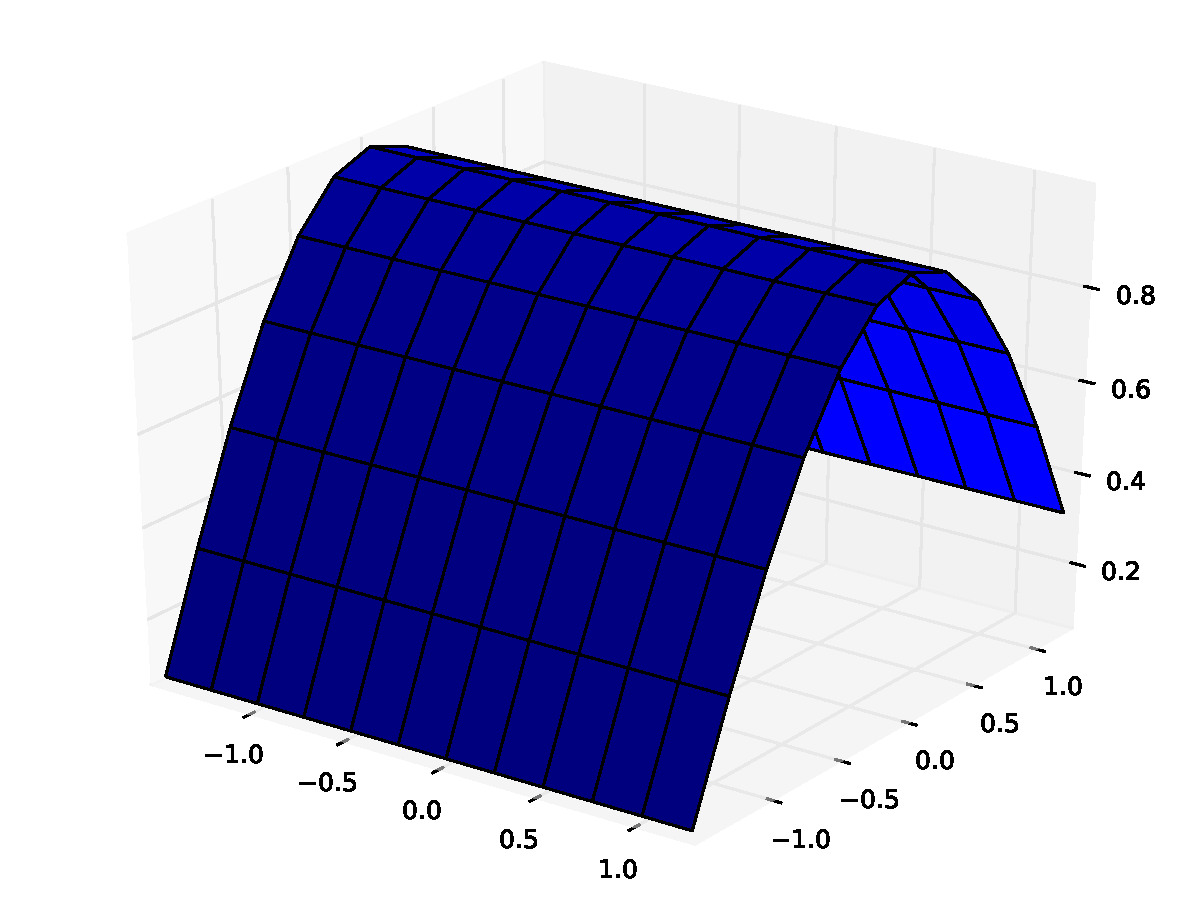
\includegraphics[scale=0.225]{figures/2d_manifold.pdf}
		}
		\end{subfloat}
	\end{center}

	\caption{Manifolds Embedded in Higher-Dimensional Space}
	\label{fig:manifolds}
\end{figure}

\section{Implications to Multi-dimensional Search}
\label{sec:implications-to-md-search}

This conjecture has implications for which index structures to use for scientific datasets. If most scientific datasets are highly sparse, they may be difficult for index structures which decompose the underlying data space without factoring in the points. For example, the Pyramid Tree uses a \textit{static} decomposition. Based on an initial boundary, exactly how the space is decomposed is already decided. This is was not a problem for the synthetic datasets used in Chapter \ref{chap:performance-evaluation}. However, there are cases where the lack of ability to \textit{adapt} the decomposition to the input data becomes problematic. This was the case with the astrophysics dataset, where the Pyramid Tree maps most points to the same few buckets.

\begin{figure}
	\begin{center}
		\begin{subfloat}[Pyramid Tree (Static)\label{fig:non-continuous-embedding}]{%
			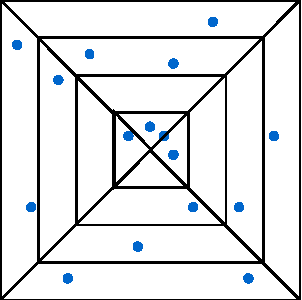
\includegraphics[scale=0.65]{figures/non_continuous_pyramid.pdf}
		}
		\end{subfloat}~~~~~
		\begin{subfloat}[Pyramid Tree (Static)\label{fig:continuous-embedding-pyramid}]{%
			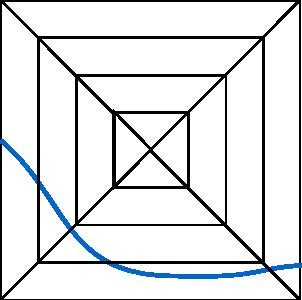
\includegraphics[scale=0.65]{figures/1d_manifold_pyramid.pdf}
		}
		\end{subfloat}~~~~~
		\begin{subfloat}[Octree (Adaptive)\label{fig:continuous-embedding-octree}]{%
			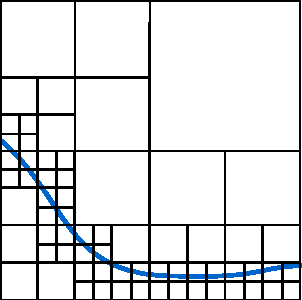
\includegraphics[scale=0.65]{figures/1d_manifold_octree.pdf}
		}
		\end{subfloat}~~~~~
		\begin{subfloat}[Multigrid (Static)\label{fig:continuous-embedding-multigrid}]{%
			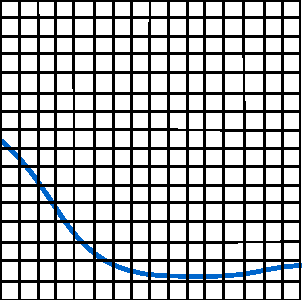
\includegraphics[scale=0.65]{figures/1d_manifold_multigrid.pdf}
		}
		\end{subfloat}
	\end{center}

	\caption{Various Spatial Decompositions of Non-Continuous 2D Dataset and 1-Manifold in 2D Space. Each Polygon Represents a Bucket}
	\label{fig:static-adaptive-decomposition}
\end{figure}

Figure \ref{fig:non-continuous-embedding} shows a dataset computed using the mapping $f : \mathbb{R}^1 \rightarrow \mathbb{R}^2$. Unlike the astrophysics dataset, $f$ is not modelling continuous physical phenomenon and is not continuous (i.e. is not a 1-manifold). This would be the case for the synthetic data randomly generated for performance analysis in Chapter \ref{chap:design-and-implementation}. In this particular example, the points are more evenly distributed across the space.

Figure \ref{fig:continuous-embedding-pyramid} shows a 1-manifold. Here, the points on the manifold will be stored in just five buckets. Without the ability to adapt, the performance of the structure will rapidly degrade as more and more points are mapped to the same few buckets.

Figure \ref{fig:continuous-embedding-octree} shows an Octree decomposition, which adapts the decomposition to provide greater discrimination between points in dense regions of space. The point $kd$-tree can be seen as an adaptive index structure to some extent, since decomposition of the underlying data space depends on the values of the given points. This is one of the reasons its performance is vastly superior to the Pyramid Tree with the two scientific datasets.

\subsection{Case Study: Multigrid}

To further support the claim that static decompositions perform poorly, we turn to the Multigrid described in Appendix \ref{chap:additional-structures}. To summarise, this index structure splits the entire data space into equal sized cells and hashes points to buckets based on the cell they are contained in. Figure \ref{fig:continuous-embedding-multigrid} shows a Multigrid decomposition of the 1-manifold discussed earlier.

The Multigrid essentially quantises continuous domains into discrete ranges which are used to hash points reliably (unlike Bit Hash) to a one-dimensional domain. The ultimate goal is to achieve perfect hashing so query times become closer to $O(d)$. The smaller the cells are made, the greater the discrimination between points there is and the smaller average bucket size will be. Theoretically, all one has to do to make the Multigrid work efficiently with the astrophysics dataset, or any dataset with dense clusters in sparse data spaces, is keep decreasing cell size until each point is in its own cell.

On real machines however, this does not work. When cells become small enough, rounding errors occur because of limited precision of floating point arithmetic. Points start being mapped to the same cell even if they are conceptually in different cells because of these rounding errors. In other words, there is a limit to how small cells can be. The astrophysics has a highly clustered distribution, with very small magnitudes for soem dimensions (e.g. $10^{-15}$). This means extremely small cell sizes are required to achieve perfect hashing and rounding errors appear very quickly.

Table \ref{tab:cell-size-effect} shows the effect of cell size on average bucket size when storing 100,000 points from the astrophysics dataset. It shows that, as you increase the number of cells for each dimension (making individual cells smaller), the average bucket size decreases. When the number of cells exceeds a certain number, which is approximately 11,000,000 per dimension for this dataset, no additional benefit is gained because the average bucket size does not change.  This shows there is a limit to how much skew static decompositions can handle, because there is a limit on how granular the decomposition can be made.	
	
\begin{table}
	\centering
	\begin{tabular}{|r|l|l|}
	\hline
	\textbf{Cells Per Dimension} & \textbf{Average Bucket Size} & \textbf{Total Buckets} \\
	\hline
	100 & 1149.43 & 87 \\
	1,000 & 168.919 & 592 \\
	10,000 & 26.5252 & 3,770 \\
	100,000 & 10.7181 & 9,330 \\
	1,000,000 & 9.10581 & 10,997 \\
	1,100,000 & 9.06454 & 11,032 \\
	1,200,000 & 9.06454 & 11,032 \\
	1,000,0000 & 9.06454 & 11,032 \\
	\hline
	\end{tabular}
	\caption{Number of Cells Used for Multigrid Index Structure and Its Effect on Bucket Size with 100,000 Astrophysics Dataset Points}
	\label{tab:cell-size-effect}
\end{table}

To summarise, adaptive decompositions allows one to quickly ``zoom in" on dense regions of points and ignore the sparse regions, even when the point distribution is not known in advance. This is something that cannot be achieved with static decompositions because of hardware limitations.

\section{Suitability of Hash-Based Approaches}
	
The Pseudo-Pyramid Tree and Pyramid Tree both produce a static decomposition of the underlying data space through the use of dimension reduction. It was shown in the empirical results from this project that the performance of these two structures is vastly inferior to the point $kd$-tree, a simple and well-established technique. These empirical results conicide with the theoretical discussion on the suitability of static decompositions for highly skewed datasets.

Adaptive variants of the Pyramid Tree exist, such as the Extended Pyramid-Technique \cite{pyramid-tree} and iMinMax($\theta$) (see Appendix \ref{chap:additional-structures}). However, the \textit{cost} of adapting such structures limits their usefulness. For example, the Extended Pyramid-Technique moves the centre of the data space to be the median of all stored points. Doing so means that the entire structure must be rebuilt because each stored point may be hashed to a different value after the centre point has moved. For large $n$ this has a massive impact on performance. An adaptable iMinMax($\theta$) was implemented in this project, but its performance was poor, despite it adapting to the dataset, because of how long rebuilding takes.

The empirical performance timings has lead this project to conclude that techniques which perform a static decomposition of the data space are \textit{not} suitable for dynamic data, unless one knows about the kinds of distributions that will be given in advance. The supplementary theoretical analysis performed in this chapter has shown that data generated by mapping continuous domains to higher-dimensional ranges are especially a challenge for structures that cannot adapt, due to the highly clustered and skewed distributions of points that result from such a mapping. Since the cost of adapting dimension reduction techniques is so high, it follows that most dimension reduction are likely to be unsuitable for dynamic data.

Despite the adaptive point $kd$-tree performing worse on highly skewed data, the structure's performance is superior to the others explored in this project. Index structures that adapt to point distributions \textit{as} points are inserted, like the point $kd$-tree, do not require an expensive rebuild procedure.

The point $kd$-tree shows that these structures can provide good performance with point queries. Existing literature often discusses how $kd$-trees degenerate to Sequential Scan with higher dimensions, but this is not the case for point queries, even with real datasets that are highly skewed.

\section{New Hypotheses}

The original hypothesis, discussed in Section \ref{sec:initial-hypothesis}, stated that the Pyramid Tree would provide faster point queries for high-dimensional scientific datasets. Based on the empirical evidence from Chapter \ref{chap:performance-evaluation} and the discussion in this chapter, the hypothesis is false. It has been abandoned in favour of the following new hypotheses.

\paragraph{\textbf{HYPOTHESIS 1:}} Most existing index structures based on reduction to a 1D value statically decompose space, and degenerate when processing highly skewed data due to floating point imprecision.

\paragraph{\textbf{HYPOTHESIS 2:}} Dimension reduction techniques cannot adapt well to skewed distributions of data because the cost of rebuilding the structure when adapting is too high.

\paragraph{\textbf{HYPOTHESIS 3:}} Dynamic tree-based structures, which adapt the decomposition of the data space as points are inserted, will generally provide better point query performance for high-dimensional scientific datasets than dimension reduction techniques.

\paragraph{\textbf{HYPOTHESIS 4:}} The Pyramid Tree is not a suitable index structure for performing point queries on skewed datasets.

\paragraph{}

The empirical evidence verifies hypothesis 4 -- the Pyramid Tree is not suitable for skewed datasets. The empirical evidence from this project, paired with the additional evaluation in this chapter, strongly supports hypotheses 1, 2 and 3. However, more research is required to verify these hypotheses.